\documentclass{imcs}
\usepackage[T2A]{fontenc}
\usepackage[utf8x]{inputenc}
\usepackage[russian]{babel}
\usepackage{graphicx}
\usepackage{hyperref}
\usepackage{enumitem}
\usepackage{listings}

\title{Реализация замыканий для языка программирования Pascal}
\author{Кевролетин Василий Владимирович}
\mentorinfo{старший преподаватель}
\mentorname{А.С.~Кленин}
\year{2013}



\begin{document}
\maketitle

\tableofcontents
\pagebreak

\section*{Аннотация}
\addcontentsline{toc}{section}{Аннотация}
Цель данной работы - реализовать поддержку замыканий в компиляторе Free Pascal Compiler.
Рассмотрены подходы к решению проблемы и осуществлена пробная реализация.

\pagebreak

\section{Введение}
\subsection{Глоссарий}

Анонимная функция -- функция, не имеющая идентификатора; доступна для
вызова либо в момент создания, либо, позднее, через ссылку на функцию,
хранящуяся в переменной.

Анонимный метод -- реализация замыканий в Delphi. 

Генератор кода -- часть компилятора, обеспечивающая создание
ассемблерного кода исходной программы по ее синтаксическому дереву.

Замыкание -- функция или ссылка на функцию вместе с используемым ею
окружением; замыкание сохраняет окружение и позволяет функции
обращаться к нему даже если она вызвана за пределами лексического
пространства где была создана.

Захваченная переменная -- переменная, используемая в теле замыкания,
объявленная во внешнем для замыкания лексическом пространстве.

Компилятор -- программа, которая считывает текст программы, написанной
на одном языке — исходном, и странслирует(переводит) его в
эквивалентный текст на другом языке — целевом.

Парсер -- часть компилятора, обеспечивающая создание синтаксического
дерева.

Свободная переменная -- пременная, используемая в теле функции, но не
являющеяся параметром этой функции. Так же встречается название
``нелокальная переменная''.

Синтаксическое дерево -- иерархическая упорядоченная структура,
состоящая из узлов, хранящих информацию об объектах, используемых в
программе.

Управляемый тип данных -- для управления памятью управляемых объектов
компилятор использует специальные техники, такие как подсчёт ссылок\cite{delhpimanged}.

Функциональное программирование -- парадигма программирования,
рассматривающая вычисление как применение математических функций,
отрицающая понятие состояния и изменяемых данных. Делает акцент на
приенении функций, а не на изменении состояния.

\subsection{Описание предметной области}

\paragraph{Free Pascal Compiler (FPC)} FPC -- компилятор языка Pascal с открытим исходным
кодом, поддерживающий несколько диалектов Pascal и генерирующий код для большого
числа процессорных архитектур и операционных систем \cite{fpc}.
Компилятор распространяется под лицензией GNU GPL. Разрабатывается
постоянной комадной добровольцев и принимает доработки от сторонних разработчиков.
Исходный код написан на языке Freepascal. Разработка ведётся с использованием системы
контрола версий SVN, системы контроля изменений Mantis. Команда общается при
помощи списков рассылки электронных писем.

Как правило, компилятор выполняет только часть работы по созданию исполняемого файла.
Широко распространённой является схема \cite{dragonbook}:
\begin{enumerate}
    \item Препроцессор.
    \item Компилятор.
    \item Ассемблер.
    \item Компоновщик.
\end{enumerate}

FPC объединяет в себе препроцессор, компилятор, и, для некоторых платформ,
компоновщик. Кроме того парсер FPC используется интегрированной средой разработки
Lazarus \cite{lazarus} TODO: link and proof.

Процесс компиляции представляет собой последовательность фаз, каждая из которых
преобразует одно из представлений исходной программы в другое. Типичное разложение
компилятора на фазы \cite{dragonbook}:
\begin{enumerate}
    \item Лексический анализ.
    \item Синтаксический анализ.
    \item Семантический анализ.
    \item Генерация промежуточного кода.
    \item Машинно-независимая оптимизация.
    \item Генерация кода.
    \item Машинной-зависимая оптимизация.
\end{enumerate}

Выдающаяся особенность FPC - поддержка нескольких диалектов Pascal 
и большого числа целевых процессорных архитекрур. Исходный код FPC написан со
стремлением минимизировать количество повторяющегося программного кода,
работающего в случае разных комбинаций
диалекта языка и результирующей платформы. Поэтому для каждой целевой платформы
в компиляторе FPC реализован отдельный генератор кода (все остальные части остаются
неизменными). В режимах совместимости с различными диалектами Pascal лексический,
синтаксический и семантический анализаторы работают немного по-разному. Благодоря этому
компилятор может иметь различную реализацию одной концепции языка в разных режимах
совместимости.

FPC находится в состоянии активной разработки. Разработчики постоянно улучшают компилятор,
добавляя новые возможности, оптимизации, поддержку новых платформ и исправляя ошибки\cite{fpc}. Одной из новых возможностей, которую разработчики и пользователи FPC хотят увидеть в
своём компиляторе, является поддержка замыканий.

\paragraph{Замыкания} В современных языках программирования замыкание это парктическая реализация
идеи лябмда-исчесления о том, что функция может использовать в своём теле свободные
переменные (не являющиеся параметрами этой функции). В лямбда-исчислении
переменные неизменяемы, поэтому для вычисления значения функции, использующей
свободные переменне, достаточно подставить значения свободных перменных в тело
функции.

В современных императивных языках программирования переменные изменяемы.
Поэтому результат выполнения функции зависит не только от значений параметров
функции, но и от значения свободных переменных, используемых в её теле. В качестве
свободных переменных могут выступать глобальные переменные и локальные переменные
других функций. Глобальные переменные доступны в течении всего времени выполнения программы.
Однако срок жизни
локальных перменных ограничен временем работы функции, в которой они объявлены.
Особенность замыканий состоит в том, они не только могут получать доступ к любым
доступным в текущем лексическом пространстве переменным, но, к тому же, могут
обращаться к ним, даже если будут вызваны в другом лексическом пространстве, где
использованные переменые уже недоступны.

Если замыкание ссылается на локальную переменную объемлящей функции, то такая перменная 
называется «захваченной»(англ. Captured)\cite{anonymmethods}\cite{cpp}. Существует 2
способа захвата переменных: по значению и по ссылке. В случае захвата по значения
замыкание в момент своего создания запоминает значение захваченных переменных.
Захват по значению - аналог подстановки значений свободных переменных в лямбда-исчислении.
В случае захвата по ссылке, в момент своего создания замыкание запоминает ссылку 
на захваченную переменную. Сложность реализации захвата переменных по ссылке состоит в том,
что на одну переменную могут одновременно ссылаться несколько замыканий и несколько
выполняющихся функций.

\subsection{Неформальная постановка задачи}

Добавить в компилятор Freepascal поддержку замыканий. В режиме совместимости с 
Delhpi реализация должна вести себя так же, как и анонимные методы
Delhpi. Дополнительно рассмотреть возможность создания альтернативной улучшенной
реализации, не ограниченной требованием совместимости с Delphi.

\paragraph{Анонимные функции}
В режиме совметимости с Delphi компилятор должен поддерживать объявление анонимных функций
в теле других подрограмм:
\begin{lstlisting}
function Factory: TProc;
begin
  Result := procedure
            begin
              Writeln;
            end;
end;
\end{lstlisting}

\paragraph{Вложенной функции}
Вложенные именованные функции должны быть реализованы в виде замыканий. Ниже пример
вложенной функции FPC.
\begin{lstlisting}    
procedure outer;
var i: Integer;

  procedure inner; begin
    i := 10;
  end;

begin
  ...
end;    
\end{lstlisting}

\paragraph{Продление жизни локальных переменных}
Без возможности захвата перменных переменная data стала бы недоступной после завершения
работы функции Factory. Каждое из созданных ниже замыканий продливает жизнь перменной
data, и может обращаться к нему даже после окончания работы Factory. В момент второго
вызова процедуры Factory переменная data, созданная во время предыдущего вызова уже
недоступна. Поэтому каждое из созданных замыканий хранит ссылку на свой собственный
экземпляр переменной data. Поэтому вызов f1() напечатает значение 10, а вызов f2()
напечатает 20.
\begin{lstlisting}
function Factory(data: Integer): TProc;
begin
  Result := procedure
            begin
              Writeln( data );
            end;
  end;
    
var f1: TProc;
begin
  f1 := Factory(10);
  f2 := Factory(20);
  f1();               { 10 }
  f2();               { 20 }
end.
\end{lstlisting}    

\paragraph{Захват по ссылке}
В языке программирования Delphi замыкания захватывают переменные по ссылке. Поэтому
позможна ситуация, когда захваченную замыканием переменную меняют из другого замыкания,
или из обычной подпрограммы. Приведённый ниже код должен напечатать значение 10.
\begin{lstlisting}
var i: Integer;
    f: TProc;
begin
  i := 0;
  f := procedure
       begin
         Writeln(i);
       end;
  i := 10;
  f();                { 10 }
end.
\end{lstlisting}

\paragraph{Захват по значению}
Рассмотреть возможность реализации захвата по значению. В примере ниже переменная
i захватывается по значению. Программа должна вывести значение 0.
\begin{lstlisting}
var i: Integer;
    f: TProc;
begin
  i := 0;
  f := procedure
       closure(i)
       begin
         Writeln(i);
       end;
  i := 10;
  f();                { 0 }
end.
\end{lstlisting}

\paragraph{Захват по значению}
Рассмотреть возможность реализации упрощенного синтаксиса для более короткого объявления
анонимных функций. В примере ниже в метод map передаётся анонимная функция, принимающая
один аргумент типа Integer и возвращающая свой аргумент, увеличенный на 1.
\begin{lstlisting}
type TListVisitor = procedure(x: Integer);
var  list: TList;
begin
   ...
   list.map(TListVisitor is x := x + 1)
   ...
end.
\end{lstlisting}

\subsubsection{Обзор существующих методов решения}

\paragraph{Аналогичные (конкурирующие) решения}

TODO: добавить JAVA, Scala
\begin{table}[h!]
\begin{center}
\begin{tabular}{|l|c|c|c|c|c|}
\hline
  ЯП     &  Анонимные  &  Вложенные  &  Захват по  &  Захват по  &  Замыкания  \\
         &  функции    &  функции    &  значению   &  ссылке     &             \\
\hline
 Perl    &  +          &  +/-        &             &  +          &  +          \\
\hline
 Python  &  +          &  +          &             &  +          &  +          \\
\hline
 Ruby    &  +          &  +          &             &  +          &  +          \\
\hline
 Scheme  &  +          &  +          &             &  +          &  +          \\
\hline
 Elisp   &  +          &  +          &             &  +          &             \\
\hline
 Scala   &  +          &  +          &  ?          &  +          &  +          \\
\hline
 Java    &  ?          &  ?          &  ?          &  ?          &  ?          \\
\hline
 C       &             &             &             &             &             \\
\hline
 C++     &  +          &             &  +          &  +          &             \\
\hline
 Delphi  &  +          &  +          &             &  +          &  +          \\
\hline
 Fpc     &             &  +          &             &             &             \\
\hline
\end{tabular}
\caption{Поддержка замыканий и анонимных функций современными ЯП}\label{tab:wsi_diff_rel}
\end{center}
\end{table}

\pagebreak

\paragraph{Описание предшествующих работ}
Студенты нашей кафедры успешно дарабатывали компилятор Fpc в рамках своих
курсовых и дипломных работ:
\begin{enumerate}
    \item Дипломная работа «Расширение компилятора Free Pascal для поддержки
обобщённого программирования». Автор Нелепа А.А. Руководитель Кленин А. С.
2007г.
    \item Курсовая работа «Анализ потоков управления для языка программирования Pascal» Автор Баль Н. В. Руководитель Кленин А. С. 2008г.
    \item Курсовая работа «Доработка компилятора Free Pascal: case of string» Автор Денисенко М. В. Руководитель Кленин А. С. 2009г.
    \item Курсовая работа «Оператор for-in для компилятора Free Pascal» Автор Лукащук М.
А. Руководитель Кленин А. С. 2010г.
\end{enumerate}

\paragraph{Вывод}
Ценность замыканий подтверждена их популярностью и востребованностью. 
Сегодня замыкания поддерживают большинство языков программирования, а программисты 
активно используют их на практике. Поэтому для поддержания компилятора FPC в 
актуальном состоянии необходимо реализовать в нём поддержку замыканий.

\subsection{План работ}

\begin{enumerate}
    \item Согласовать план работ с разработчиками FPC.
    \item Изучить архитектуру и исходных код компилятора.
    \item Изучить реализацию замыканий в похожих языках программирования.
    \item Спроектировать реализацияю.
    \item Осуществить пробную реализацию.
    \item Используя полученный опыт создать окончательную реализацияю.
\end{enumerate}

\section{Требования к окружению}

FPC может компилировать свой собственный исходный код. Поэтому
список целевых платформ совпадает со списком платформ, на которых работает
FPC.

\subsection{Требования к аппаратному обеспечению}

Для работы требуется компьютер, пригодный для набора исходного кода программы.
Т.е. кроме работающих процессора, оперативной и постоянной памяти требуются
клавиатура и монитор.

Поддерживаемые архитектуры процессоров\cite{fpctargets}:
\begin{itemize}
    \item I386
    \item PowerPC
    \item Sparc (initially working, lots of additional work done)
    \item AMD64 (x86-64)
    \item PowerPC64
    \item ARM
    \item m68k 
\end{itemize}

\subsection{Требования к программному обеспечению}

\paragraph{Компилятор} FPC версии 2.6 и выше
\paragraph{Операционная система}
На сайте FPC указано 53 разных поддерживаемых комбинаций архитекруты 
процессора и операционной системы\cite{fpctargets}. Здесь приведём
только популярные операционные системы, поддерживаемые компилятором
для архитектуры процессора I386:
\begin{itemize}
    \item Win32 for i386
    \item Linux for i386
    \item Target Darwin (Mac OS X) for i386 (2.1.x and later)
    \item FreeBSD/ELF for i386
    \item Android for i386
\end{itemize}
    
\subsection{Требования к пользователям}
Программисты, владеющие языком программирования Free Pascal или Delphi.

\section{Архитектура системы}

С точки зрения пользователя проект компилятора FPC состоит из нескольких 
частей:
\begin{description}
    \item[Сompiler] - программа с интерфейсом командной строки. На вход
принимает список текстовых или объектных файлов. Результат работы --
файлы с ассемблерным кодом, описанием модулей, отладочной инфомрацией,
информацией для межмодульной оптимизации и исполняемый файл.
    \item[Ide] - среда разработки с интерфейсом командной строки.
    \item[Installer] - скрипты для установки программы в систему.
    \item[Packages] - стандартная библиотека, состоящая из опциональных
библеотек, не обязательных для работы скомпилированной программы.
    \item[Rtl] - библиотека времени исполнения, содержащая код вспомагательных
подпрограмм, необходимых для работы любой скомпилированной программы. К 
примеру, менеджер динамической памяти и подпрограммы управления памятью
управляемых объектов реализованы здесь.
    \item[Tests] - набор тестов.
    \item[Utils] - вспомогательные утилиты, не используемые компилятором,
но полезные пользователю. К примеру, содержит утилиту ppudump, переводящую
содержимоей файла описания мудуля, в тектовый формат.
\end{description}

Несмотря на то, что для конечного пользователя компилятор - это монолитная
программа, преобразующая файлы из одного представления в другое, в рамках
данной работы необходимо рассмотреть внутреннюю архитектуру самого компилятора.
Это необходимо для обоснования принятых решений, последствия которых 
испытают конечные пользователи. К таким решениям относятся, к примеру,
размер указателя на замыкание, либо правила управления памятью,
выделенной под замыкания.

\subsection{Архитектура компилятора}

Весь программный код можно условно раздилить на начальную стадию(англ. front-end)
и заключительная стадию(англ. back-end)\cite{dragonbook}.

Начальная стадия считывает входные данные, проверяет их на корректность, строит
вспомогательные структуры данных, необходимые для генерации кода и передаёт 
управление заключительной стадии, которая генераторует код.

Смысл разделения на начальную и заключительную стадию в
том, чтобы отделить детали анализа языков высокого уровня от деталей,
относящихся к целевой архитекруре. Такой подход позволяет уменьшить сложности
одновременной поддержки несколько диалектов Pascal и большого числа целевых
архитектур.

\subsubsection{Начальная стадия}

После запуска FPC обрабатывает параметры и проводит предварительную обработку
исходного кода входной прогрммы. Далее он целиком считывает определение и тело
одной подпрограммы, проводит неоходимые проверки и генерирует для неё
код высокоуровнего ассемблера. Затем считывает слудующую подпрограмму и так далее
до конца файла.

Обработка одной подпрограммы на начальной стадии включает в себя:
\begin{enumerate}
    \item Лексический анализ.
    \item Синтаксический анализ.
    \item Семантический анализ.
    \item Машинно-независимую оптимизацию.
\end{enumerate}

Операции, производимые любым компилятором можно реализовывать в виде
отельных проходов по синтаксическому дереву или потоку лексем. К примеру, можно
полностью считать лексемы входного файла и получить поток лексем. Затем запустить
синтаксический анализ и получить синтаксическое дерево, соответствующее содержимому
файла. Затем семантический анализ, который не производит никаких модификаций и 
лишь проверяет синтаксическое дерево на корректность. И лишь потом производить
преобразования синтаксического дерева.

Описанная выше схема уменьшает сложность компилятора. Программу в которой отдельные 
компоненты совершают чётко определённые действия легко документировать и понимать.
К сожалению многократный обход структур данных вносит накладные расходы, поэтому
зачастую несколько отдельных проходов объединяют в один. В компиляторе FPC стадии
лексического, синтаксического и семантического анализа реализованы в виде одного
прохода. 

Кроме того, стадия семантического анализа, кроме вывода типов и проверки синтаксического
дерева на корректность, производит вспомогательные модификации синтаксического дерева.
FPC на этапе семантического анализа добавляет преобразования типов, заменяет операции
с управляемыми данными на вызовы функций из библеотеки времени выполнения и преобразует
некоторые специфичные конструкции (к примеру для загрузки адреса процедуры используется
специальный узел синтаксицеского дерева, отличный от того, который создает парсер).

\subsubsection{Синтаксическое дерево}

Синтаксическое дерево - структура данных представляющая иерархическую синтаксическую
структуру исходной программы\cite{dragonbook}. После синтаксического анализа каждый внутренний узел 
дерева представляет собой оператор, дочерние узлы представляют собой операнды этого
оператора. Для представления синтаксического дерева и операций над ним FPC использует
приём объектно-ориентированной декомпозиции. В \cite{gof} такой подход описан под
названием "compisite"(англ. составной).

Все узлы синтаксического дерева унаследованы от одного абстрактного класс tnode.
tnode объявляет общий интерфейст для объектов синтаксического дерева. Унаследованные
от tnode классы, реализуя этот интерфейс, определяют специфичное поведение. Отметим
методы, реализующие обходы синтаксического дерева:
\begin{itemize}
    \item pass\_1 -- выделение регистров;
    \item pass\_typecheck -- семантический анализ;
    \item pass\_generate\_code -- генерация кода.
\end{itemize}

На диаграмме показано, как использование наследования позволяет отделить общие для 
нескольких синтаксических конструкций детали от специфичиных деталей отдельной конструкции.
Так, tunarynode служит базовым классом для всех операций, содержащих 1 операнд.
Унаследованный от него класс tloadvmtaddrnode реализует методы pass\_1 и pass\_typecheck,
которые реализованы без использования информации о целевой архитектуре. Метод
генерации кода pass\_generate\_code реализован в классе \\ tcgloadvmtaddrnode.

Таким образом, для каждой архитектуры процессора можно реализовать отдельный класс, 
унаследованный от tloadvmtaddrnode и реализовать генерацию кода, 
учитывая особенности конкретного процессора.
Такой подход к модификации поведения объекта, переопределяя методы родительского классса,
описан в \cite{gof} под названием "template"(англ. шаблон). Этот подход широко
используется в FPC для отделений специфичных деталей генерации кода узлов синтаксического
дерева от от остальной логики.

\begin{figure}[htb]
\centering
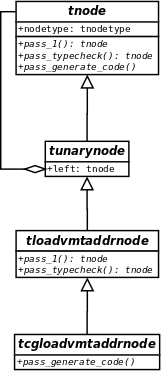
\includegraphics[width=150px]{./uml/cgnodeexample.png}
\caption{Диаграмма наследования для класса tcgloadvmtaddrnode}
\end{figure}

\subsubsection{Таблицы сомволов}

TODO: Таблицы символов содержат информацию о именованных объектах, встречающихся в 
программе. Это модули, типы, переменные, константы, подпрограммы. Мы планируем
генерировать не просто только синтаксическое дерево, но и целые типы данных! Такое
явление встречается в природе - для доступа к локальным переменным объемлящих процедур
в JVM, FPC складывает провинившиеся локальные переменные в структурку и передаёт её в
качестве типизированного аргумента(а не void*, как в простонародье). Так есть
проблема с тем, что в JVM нет адресной арифметики.

\subsubsection{Трансформации синтаксического дерева}

Во время компиляции FPC неоднократно трансформирует полученное на этапе синтаксического 
анализа синтаксическое дерево. Это необходимо для:
\begin{itemize}
    \item Упрощения логики отдельных узлов синтаксического дерева. К 
примеру, узлы преобразования типов упрощают логику узлов загрузки значения переменных,
арифметических операций и др. выражений.
    \item Проведения машинно-независымой оптимизации. К примеру удаление недостижимого
кода.
    \item Реализации новых концепций языка через старые. К примеру, реализация
case of string\cite{misha} или доступ к локальным переменным объемлящей функции в
случае компиляции в байт-код.
\end{itemize}      

Возможность реализации новых концепций языка через старые можно использовать и
для реализации замыканий. Заметим, что замыкание отличаются от 
обычный подпрограммы наличием свободных переменных. Преобразование
замыкания в процедуру, не содержащую свободных переменных называется преобразованием
замыканий\cite{moderncompiler}.

Преобразование замыканий давно используется в языках программирования, основанных на
лямбда-исчислении. Прямая реализация модели подстановки
лямбда-исчисления приводит к многократному вычислению одних и тех же веражений.
Преобразованием замыканий позволяет избежать бесполезных вечислений
и улучшения производительности таких программ \cite{lambdaclosure95}. 
Функция со свободными переменными
заменяются фуцией с дополнительными параметром - окружением. Свободные переменыне
в теле исходной функции заменятся ссылками на окружение.  
Неизменяемость переменных в лямбда-исчислении позволяет реализовать сохранение
переменных в окружение разными способами:
\begin{description}
    \item[Общее окружение] Замыкания, имеющие общие свободные переменные,
используют общее окружение. Во время выполнения программы по мере активации функций
из вновь созданных окружений необходимо составлять связный список.
Преемущество такого подхода - быстрое создание окружения и экономия памяти. Недостатком
является увеличение времени доступа к переменным, т.к. время доступа к элементам связного
списка пропорционально длине списка.
    \item[Плоское окружение] Для каждого замыкания создаётся отдельная структура данных,
содержащая значения всех необходимых переменных. Плюс такого подхода - быстрый доступ
к переменным окружения. Минус - долгое создание замыкания и дополнительный расход памяти.
\end{description}

Описанный подход преобразования замыканий применим к императивным языками
программирования. Статически типизированный язык программирования Scala
использует преобразования замыканий\cite{scalaoverview}\cite{scalaclosure}. То что
Scala использует статическую типизацию и допускает изменение переменных делает
язык очень похожими на Free Pascal. Главное отличие - полностью автоматическое
управление динамической памяти компилятором, решающее проблему управления памятью
созданных окружений.

\subsubsection{Заключительная стадия}

В FPC нет промежуточного представления кода, который начальная стадия
передавала бы в заключительную стадию. Вместо генерации промежуточного представления
узлы синтаксического дерева последовательно вызывают методы высокоуровневого генератора
кода. Такой подход очень похож на использование промежуточного представления, но
избавляет от необходимости генерировать промежуточные структуры данных.

TODO: что ли расскажи почему генератор высокоуровневый и зачем тут няшная диаграмма.

\begin{figure}[htb]
\centering
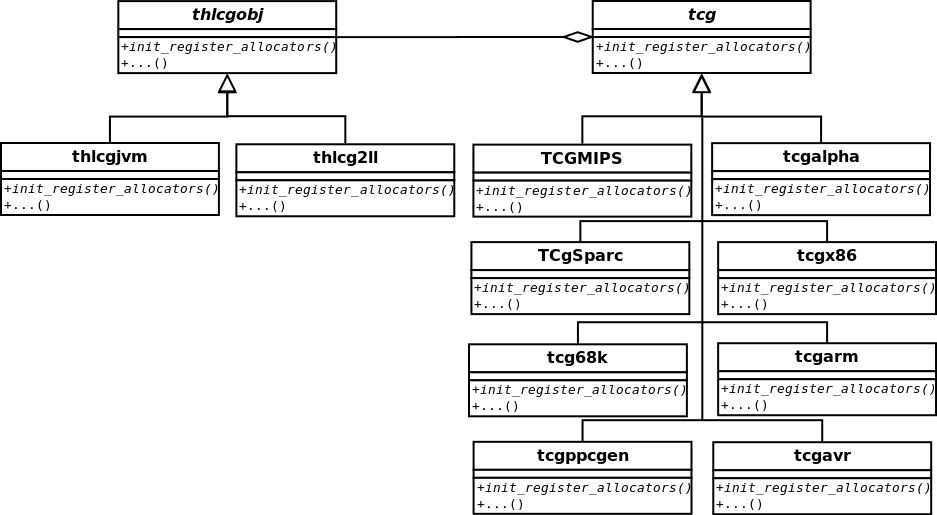
\includegraphics[width=\textwidth]{./uml/cgen.png}
\caption{Диаграмма классов генератора кода}
\end{figure}

\section{Функциональные требования}
Компилятор должен:
\begin{enumerate}
    \item Сохранить обратную совместимость. Он должен проходить существующие тесты. 
    \item В режиме совместимости с Delphi корректно компилировать программы,
содержащие замыкания, которые компилирует Delphi.
    \item В остальных режимах предоставить пользователям использовать замыкания,
возможно с расширенными набором возможностей и альтернативным синтаксисом.
\end{enumerate}
        
\section{Требования к интерфейсу}

Компилятор имее интерфейс командной строки, который описан
в руководстве пользователя FPC\cite{userguide}. Интерфейс остаётся неизменным.

\section{Проект}

\subsection{Средства реализации}

Проект использует язык программирования Free Pascal. Редактирование исходных кодов
компилятора возможно с использованием любого текстового редактора. Тем не менее
для работы с проектом большого размера предпочтительно использование редактора с
поддержкой навигации по коду. Возможность быстрого перехода к объявлению и описанию
идентефикаторов упрощает поиск нужной информации и ускоряет процесс разработки.
Было рассмотрено несколько кандидатов:
\begin{description}
  \item[Free Pascal's text mode IDE] Приемущества: находится в репозитории с 
компилятором. Недостатки: отсутствует графический интерфейс, отсутствует
быстрый переход к определению переменных.
  \item[Emacs] Приемущества: можный текстовый редактор, поддерживающий большое
количество расширений. Недостатки: переход к определению переменных не работает
с исходными кодами FreePascal.
  \item[Lazarus] Приемущества: удобный графический пользовательский интерфейс.
Корректный быстрый переход к определению символов. Настраиваемые горячие клавиши.
В репозитории компилятора есть файл проекта для Lazarus.
  \item[MSEide] Примемущества: быстрый. Недостатки: неудобный 
пользовательский интерфейс.
\end{description} 
В итоге было принято решение использовать среду разработки Lazarus, так как она
лучше всего подходит для работы с большим проектом. Lazarus корректно разбирает
исходный код на языке программирования FreePascal и предоставляет пользователю
возможность удобной и быстрой навигации по коду.

\subsection{Структуры данных}

TODO:

\subsection{Модули и алгоритмы}

TODO:

\subsection{Стандарт кодирования}

Стандарт кодирования описан в документации проекта.\cite{codingstyle}:
\begin{itemize}
  \item Ключевые слова пишутся маленькими буквами.
  \item Символы табуляции запрещены.
  \item Не следует отделять операторы, запятые и скобки пробелами.
  \item Размер отступов: 2 пробела для каждого уровня отступа.
  \item Перед блоком begin ... end следует делать отступы.
  \item Подпрограммы разделяют двумя пустыми строчками.
  \item У идущих подруд условных операторов следует писать else и последующее if 
на одной строке.
\end{itemize}

\section{Реализация и тестирование}

\pagebreak

\section*{Заключение}
\addcontentsline{toc}{section}{Заключение}

Таким образом в процессе выпонения дипломной работы мною были углублены
знания о компиляторах современных языков программирования, улучшены навыки
поддержки и развития больших программных проектов. Я получил опыт участия в 
международном проекте с открытым исходным кодом и пообщался с опытними разработчиками.
Мною была рассмотрены различные общие подходы к реализации замыканий и разработано
решение для конктреного компилятора FPC.

Итогом работы стала пробная реализация, позволившая оценить сложность реализации 
замыканий, положительные и отрицательные черты выбранного подхода.
Созданная реализация должна
стать прототипом для окончательной понятной, стабильной и задокументированной
реализации замыканий для компилятора FPC.

\pagebreak

\begin{thebibliography}{99}
\bibitem{misha} Курсовая работа «Доработка компилятора Free Pascal: case of string». Автор Денисенко М. В. Руководитель Кленин А. С. - 2009г.
  
\bibitem{fpc} Free Pascal Compiler \url{http://www.freepascal.org/}
\bibitem{dragonbook} Альферд~В.~Ахо, Моника~С.~Лам, Рави~Сети, Джеффри~Д. Ульман. Компиляторы. Принципы, технологии и инструментарий. - 2 изд. - Вильямс, 2008. - 1184 с.
\bibitem{moderncompiler} Andrew~W.~Appel. Modern Compiler Implementation in Java. - 2nd edition - Cambridge University Press, 2004. - 512с.
\bibitem{engineeringcompiler} Keith~D.~Cooper, Linda Torczon. Engineering a Compiler. - 2nd edition - Morgan Kaufmann Publishers, 2012. - 801c.
\bibitem{cpp} Standard for Programming Language C++ \url{http://www.open-std.org/jtc1/sc22/wg21/docs/papers/2012/n3485.pdf}
\bibitem{lambdaclosure95} Yasuhiko~M., Greg~M., Robert~H. Typed  Closure Conversion. - Carnegie Mellon University, 1995. - 40c.
  
\bibitem{anonymmethods} Документация Delphi: Anonymous methods \url{http://docwiki.embarcadero.com/RADStudio/XE3/en/Anonymous_Methods_in_Delphi}
\bibitem{delhpimanged} Документация Delphi: System.Rtti.IsManaged \url{http://docwiki.embarcadero.com/Libraries/XE4/en/System.Rtti.IsManaged}
\bibitem{fpctargets} Freepascal Wiki: Platform list \url{http://wiki.freepascal.org/Platform_list}
\bibitem{scalaclosure} Miguel Garcia. Code walkthrough of the UnCurry phase (Scala 2.8). Hamburg University of Technology, 2009г. - 5с.
\bibitem{scalaoverview} Martin Odersky and others. An Overview of the Scala Programming Language. - 2nd edition - Ecole Polytechnique Federale de Lausenne, 2001г. - 20c.
\bibitem{gof} Гамма~Э., Хелм~Р., Джонсон~Р., Влиссидес~Д. Приемы объектно-ориентированного проектирования. Паттерны проектирования, Спб.:Питер, 2010, 386 c.
\bibitem{userguide} Michaël Van Canneyt, Florian Klämpfl. Free Pascal : User’s Guide. 2013 \url{http://www.freepascal.org/docs-html/user/user.html}
\bibitem{codingstyle} Free Pascal Documentation. Coding style \url{http://wiki.freepascal.org/Coding_style}
  
Обсуждениe Delphi anonymous methods в списке рассылок разработчиков fpc (fpc-devel):

\bibitem{sven1} Sven's comment - \url{http://lists.freepascal.org/lists/fpc-devel/2013-March/031595.html}
\bibitem{Marko1} Marko's comment - \url{http://lists.freepascal.org/lists/fpc-devel/2013-March/031657.html}
  
\end{thebibliography}
\addcontentsline{toc}{section}{Список литературы}

\pagebreak

\noindent Автор работы \superunder{\hrulefill}{\hspace{2cm}(подпись)\hspace{2cm}} (Ф.И.О.)\\

\noindent{}Квалификационная работа допущена к защите\\

\noindent{}Назначен рецензент\\
\superunder{\hrulefill}{(Фамилия, И.О. рецензента, ученая степень, ученое звание)\hspace{5cm}}\\

\vspace{2\baselineskip}
\noindent\begin{tabular}{p{0.5\textwidth} p{0.45\textwidth}}
\parbox{8cm}{Зав. кафедрой информатики,\\ математического и компьютерного\\ моделирования} &
\hfill А.~Ю.~Чеботарев\\
\end{tabular}
\vspace{2\baselineskip}
\begin{flushright}
Дата <<\rule{1cm}{0.5pt}>>\rule{3cm}{0.5pt}\quad 2013 г.
\end{flushright}

\end{document}